\appendix
\label{sec:appendix}

\subsection{Ethics}
This work does not raise any ethical issues.
% following https://conferences.sigcomm.org/imc/2025/submission-instructions/

\subsection{Additional background information}
\textbf{\gls{CT} logs.}
\gls{CT} is a protocol for logging TLS certificates to support monitoring and auditing. The \glspl{CA} submit issued certificates to the public, append-only logs, with the intent to track \glspl{CA} behavior and spot suspicious certificates. Browsers (\eg Google) and \glspl{CA} (\eg Let's Encrypt) operate these logs.
However, the CA/Browser Forum has not made \gls{CT} mandatory.
\openintel continuously retrieve and archive certificates from \gls{CT} logs. The resulting \dataset includes billions of unique certificates.
%Domain names that appear in the certificate's Common Name and Subject Alternative Name fields allow us to use as a basis for our \gls{DNS} scans on \gls{DMARC} records.\verbose\rhl{I doubt this is necessary.}

\textbf{Incentives for DMARC adoption.}
\gls{DMARC} adoption is influenced by different factors. First, governments and registries from \gls{ccTLD} issue technical guidelines that can impact the adoption of \gls{DMARC}. Governments, often through their cybersecurity agencies, publish their recommendations that cover national governmental domains as well as private sectors and individuals~\cite{_BSITR03182Email_,_SecuringGovernmentEmail_2024,ccn-cert-es}.
The registries are responsible for maintaining a zone file for the \gls{TLD}, and misuse of domain names can affect \gls{TLD}'s reputation. Therefore, some registries advises security policies to improve the overall security posture of their \gls{TLD} with \gls{DMARC}~\cite{_Report2023Ch_,_GermanysBSIPublishes_}.
The incentive can extend beyond financial benefits for domain owners who use \gls{DMARC}~\cite{_Report2023Ch_}.
Additionally, governments and \gls{ccTLD} registries may reference documents from other countries as a starting point for further improving their own policies~\cite{_GermanysBSIPublishes_}.

Second, beyond governments and registries, industry regulations also drive \gls{DMARC} adoption. For example, since February 2024, Google and Yahoo started requiring bulk email senders to implement \gls{DMARC}~\cite{_NewGmailProtections_2023,_Yahoo_2023}, and Microsoft followed a similar approach in May 2025~\cite{_StrengtheningEmailEcosystem_}. These requirements ripple across the ecosystem, with other providers following and extending them to all email senders, regardless of volume~\cite{_AideLignePostmaster_,_EmailDomainAuthentication_}.
Such practices reflect the alignment among email providers to protect users from phishing campaigns.

Finally, the ecosystem supporting domain owners, from hosting providers to consortia, amplifies the \gls{DMARC} adoption. Many hosting providers offer built-in, user-friendly interfaces to simplify configuring \gls{DMARC} with online tutorials~\cite{_GoDaddyWatDKIM_,_AuthenticateYourDomain_}.
The M3AAWG, a global anti-abuse consortium, provides guidelines and best practices to deploy \gls{DMARC}~\cite{m3aawg2020}. Since June 2024, the PCI Security Standards Council, a global forum that helps drive the adoption of security standards and resources for safe payments, included \gls{DMARC} in its compliance framework~\cite{pci2024}.
Together, these actors lower the technical barrier and help normalize the use of secure email.

\subsection{Analysis tools}
Our data analysis tools are at \textit{\url{github.com/internettransparency/dmarc-cctld-research}} under a permissive license.

\subsection{Additional view on DMARC reporting}
\label{subsec:sankeys}
Additional view on destination mailboxes receiving \gls{DMARC} reports.
\begin{figure}[ht]
    \centering
    \begin{subfigure}{0.48\textwidth}
        \centering
        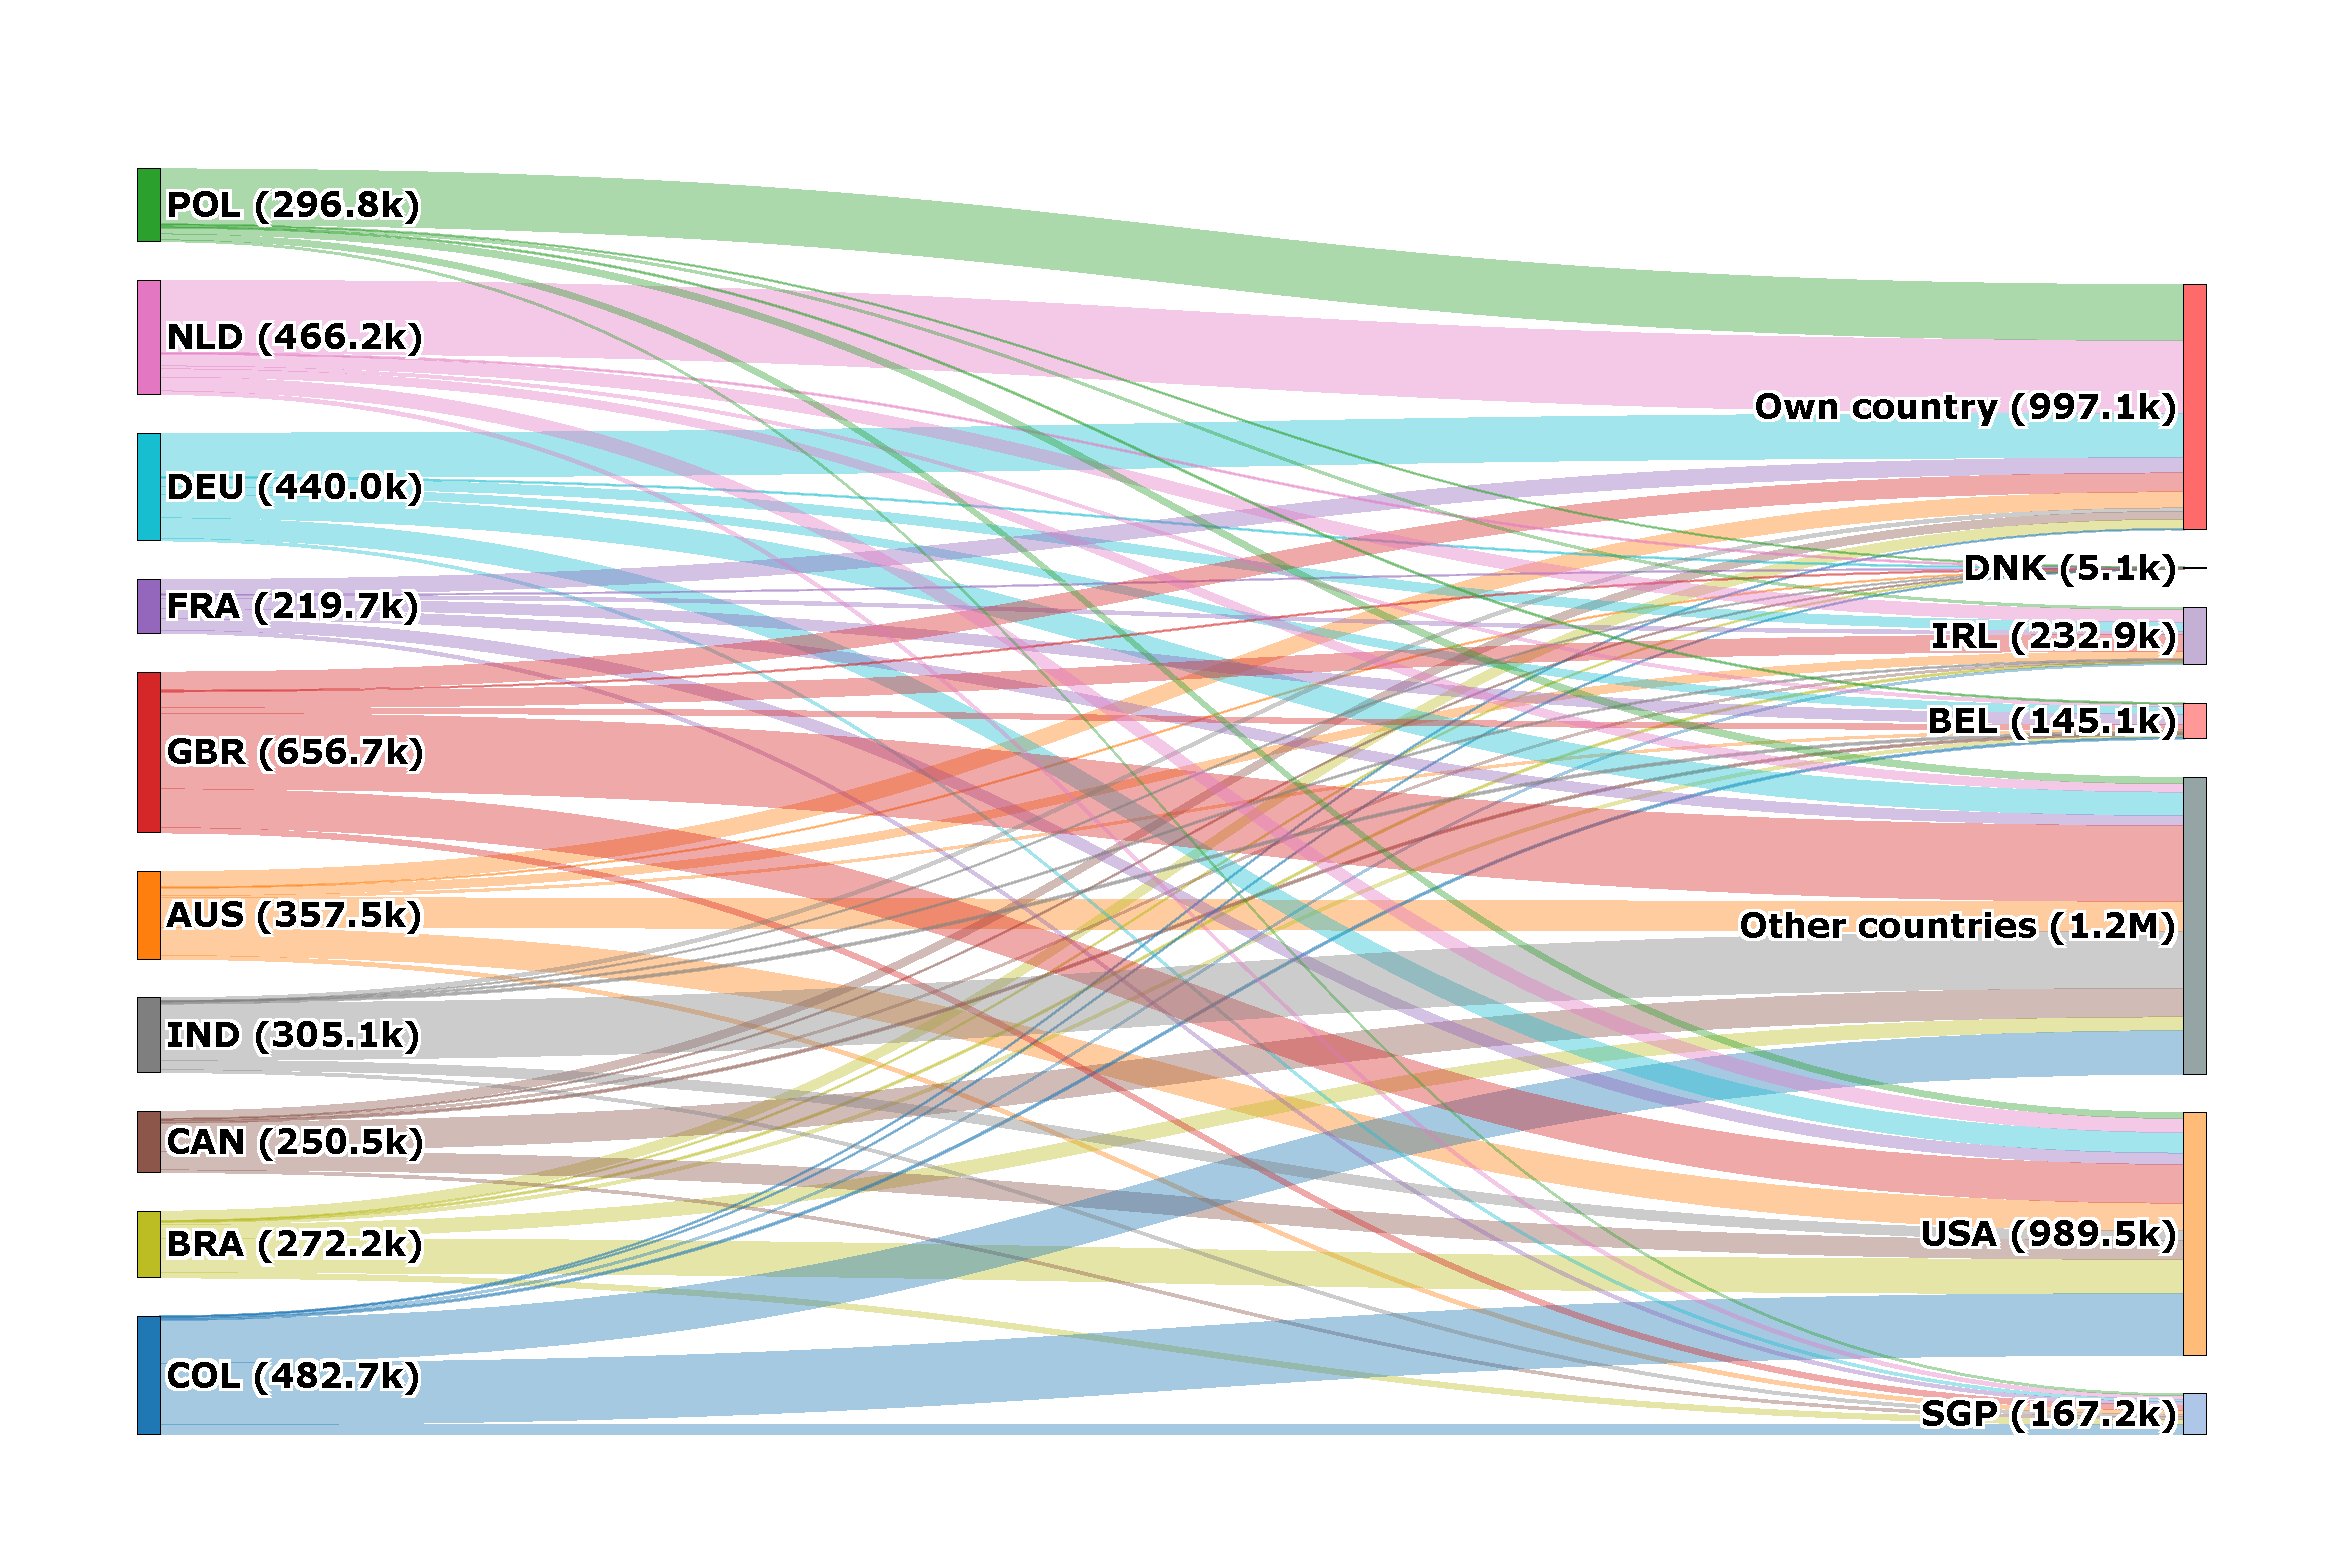
\includegraphics[width=\linewidth]{figures/countryxcountry_sankey.pdf}
        \caption{All ccTLDs.}
        \label{fig:countryxcountry_sankey}
    \end{subfigure}
    \hfill
    \begin{subfigure}{0.48\textwidth}
        \centering
        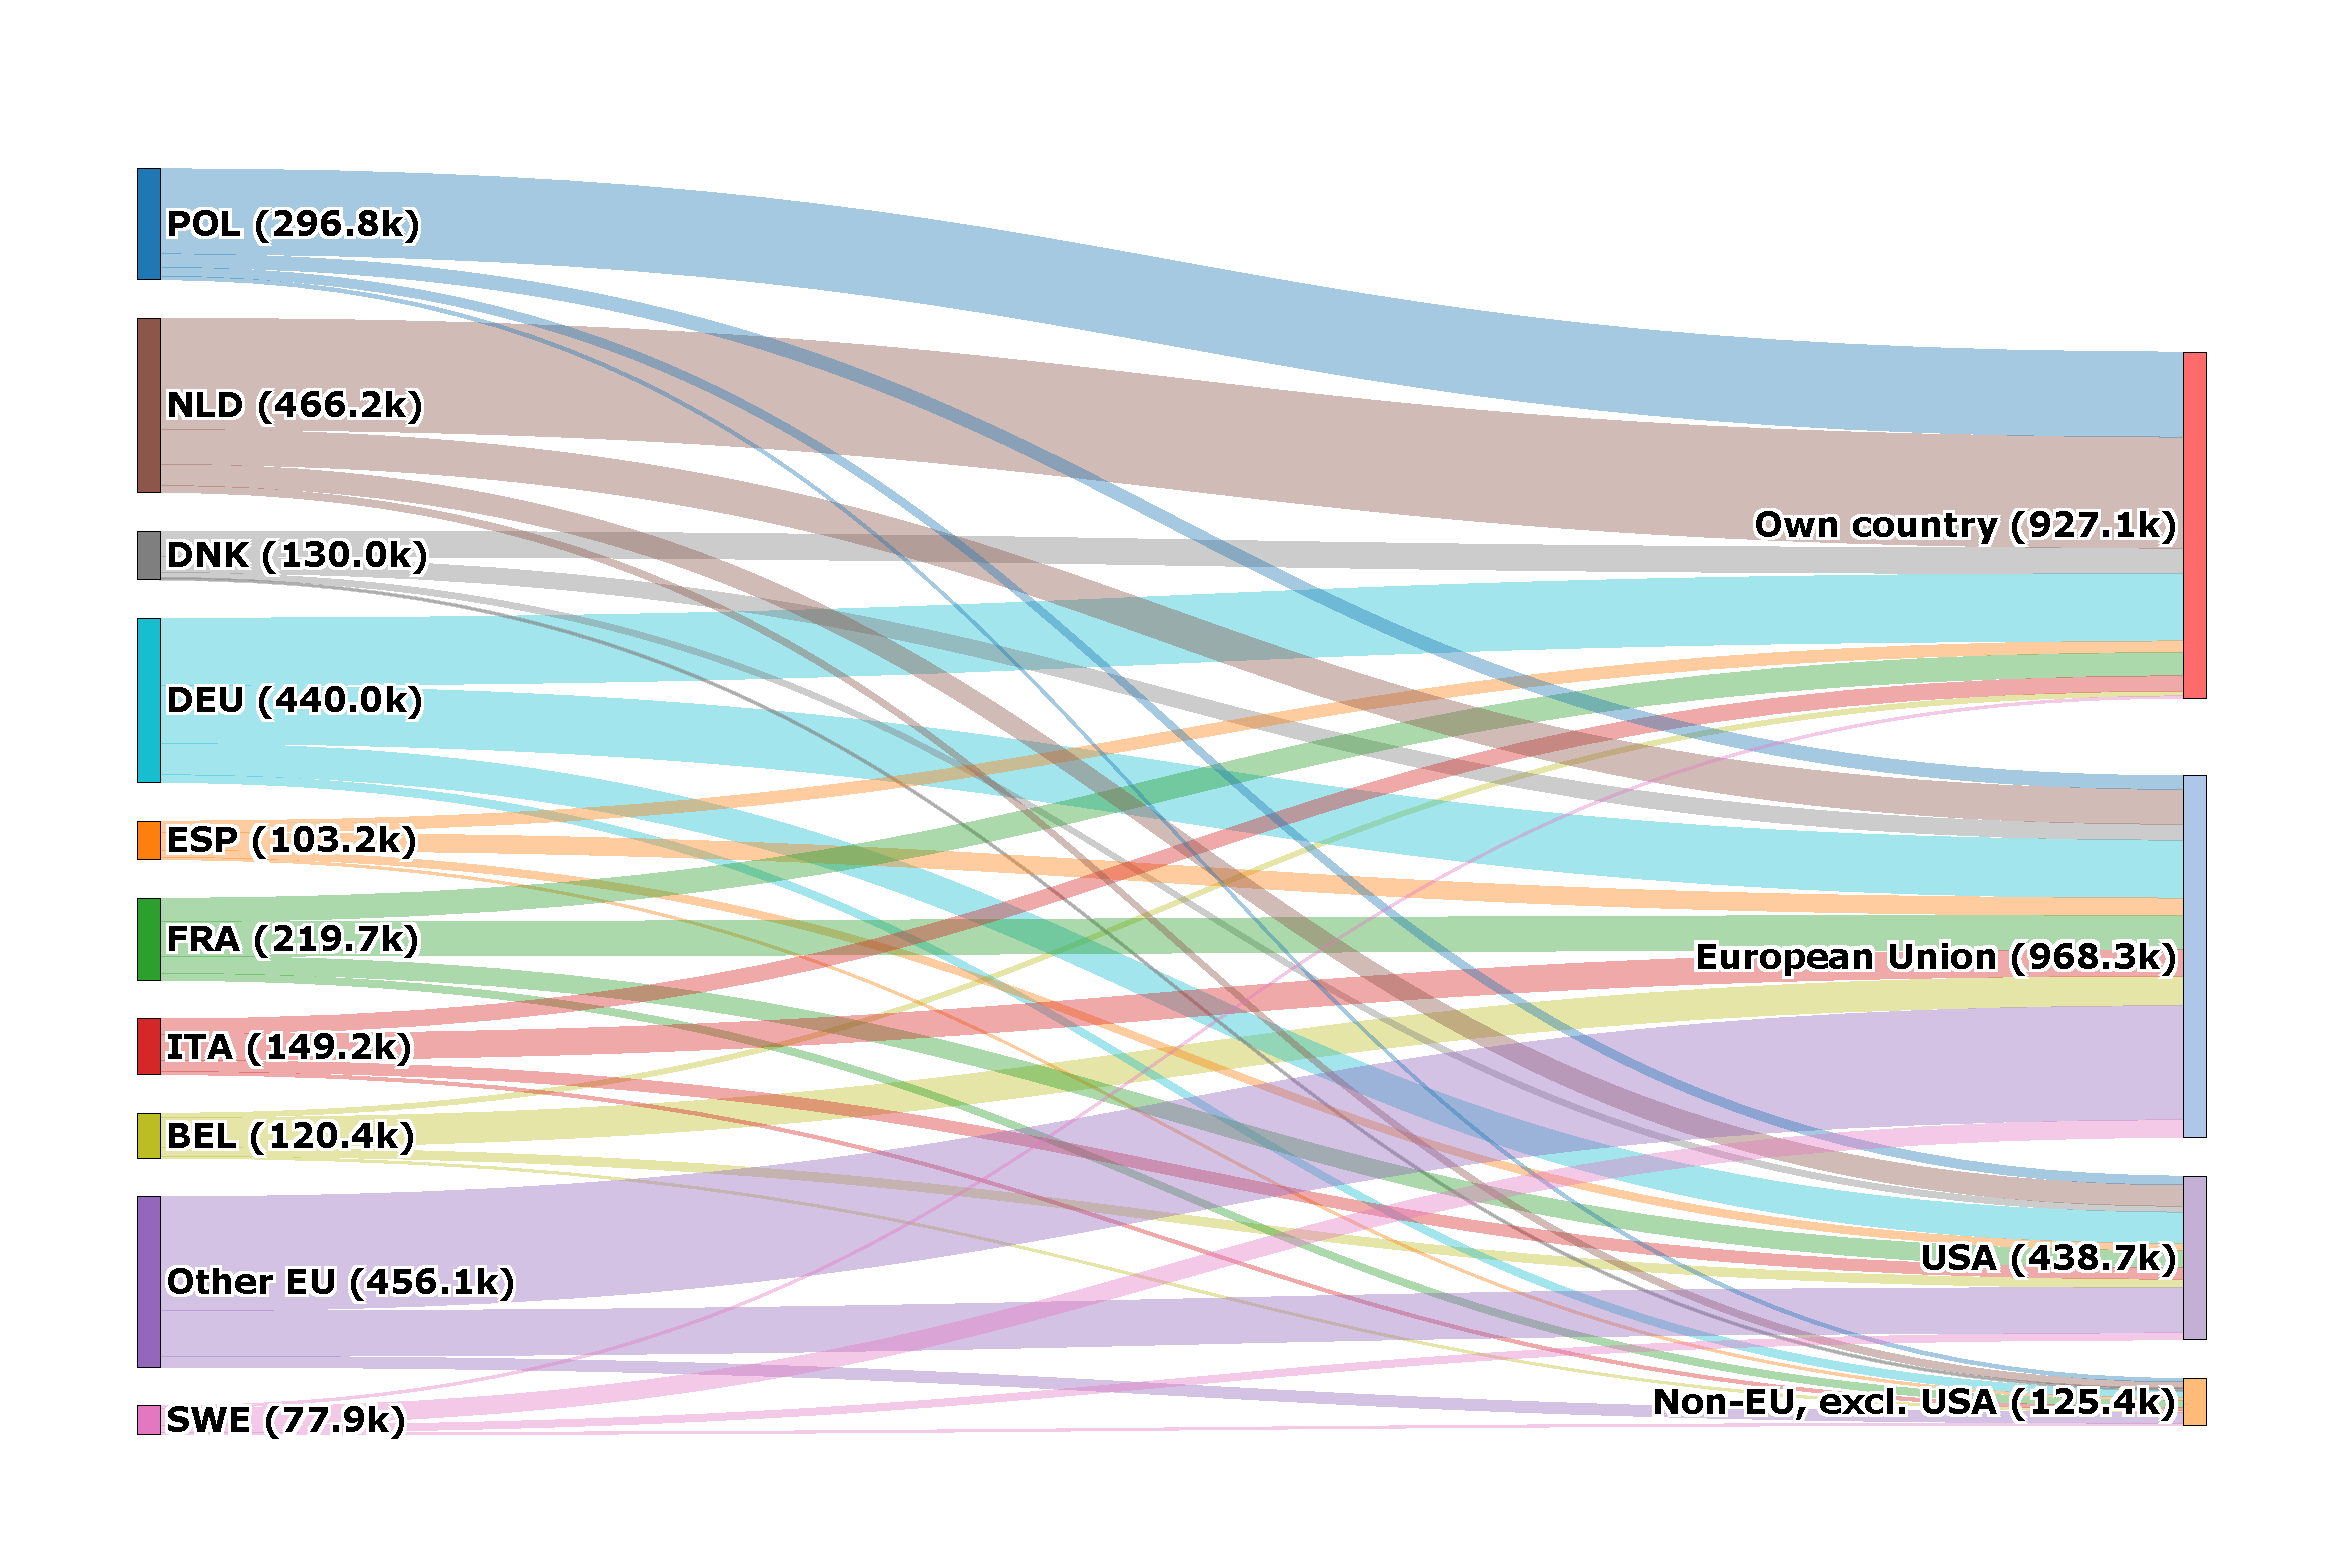
\includegraphics[width=\linewidth]{figures/EU_countryxcountry_sankey.pdf}
        \caption{European Union domains.}
        \label{fig:EU_countryxcountry_sankey}
    \end{subfigure}
    \hfill
    \begin{subfigure}{0.48\textwidth}
        \centering
        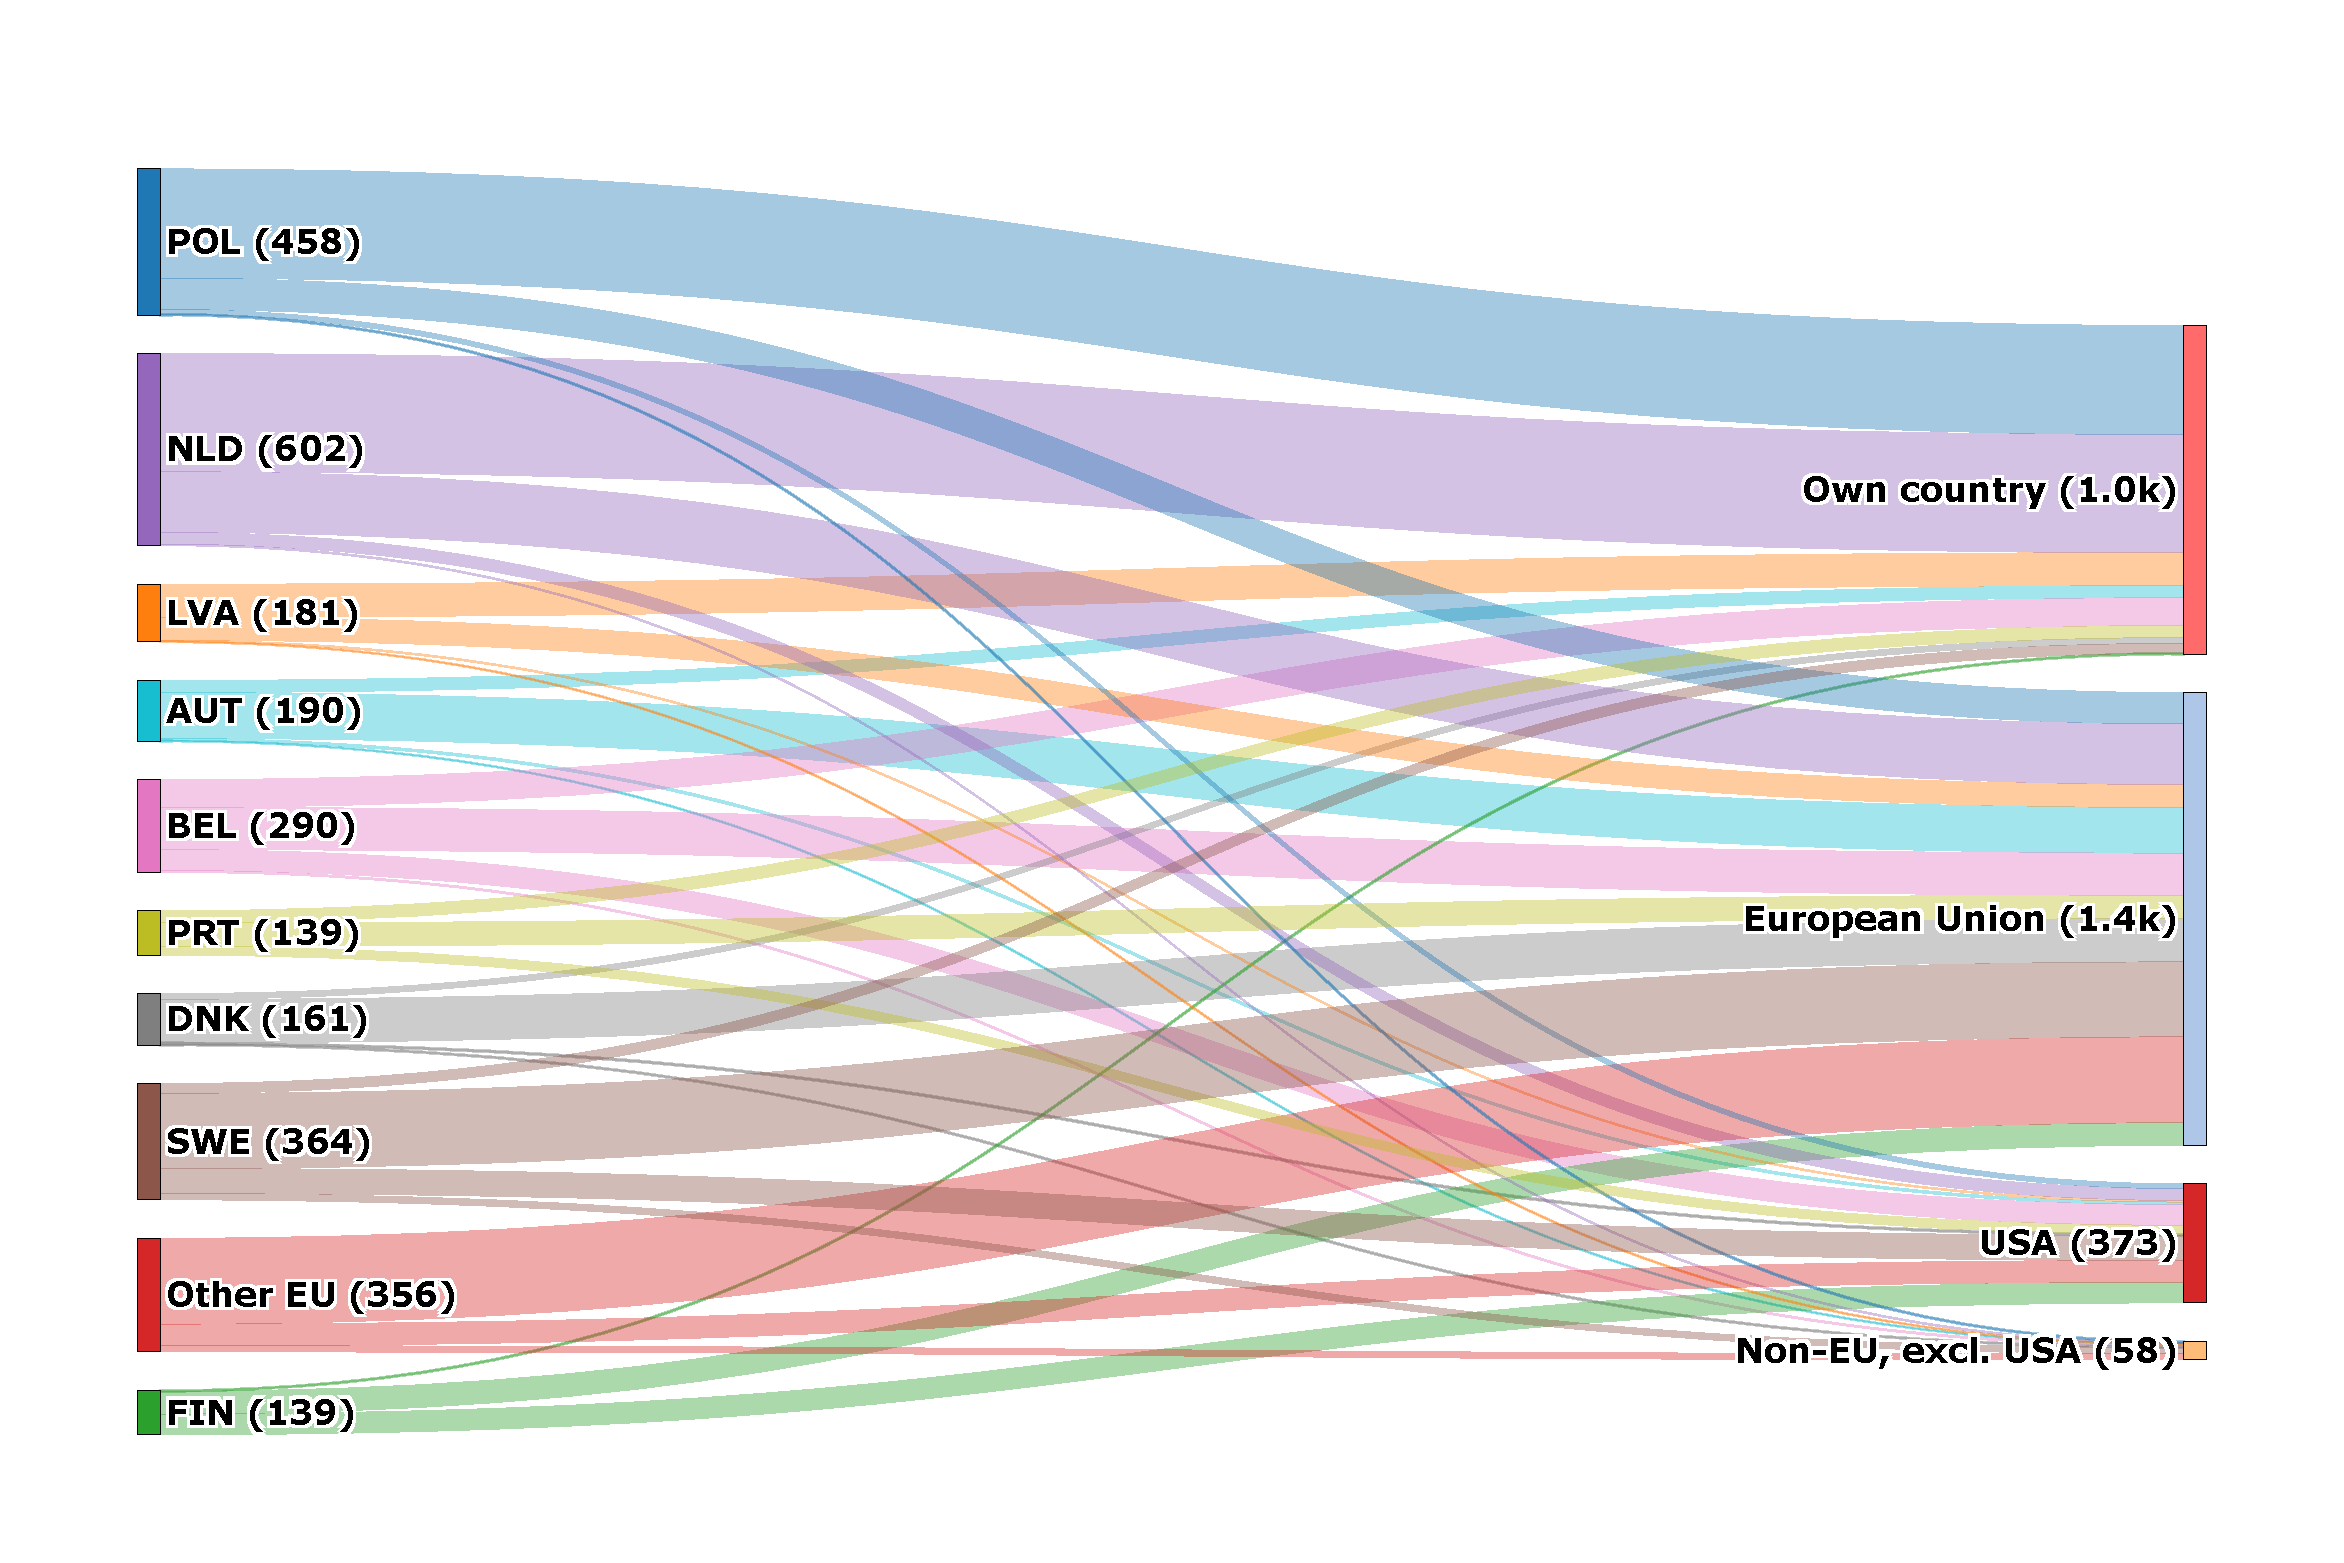
\includegraphics[width=\linewidth]{figures/EU_gov_countryxcountry_sankey.pdf}
        \caption{European Union governmental domains.}
        \label{fig:EU_gov_countryxcountry_sankey}
    \end{subfigure}
    \caption{Sankey diagram of DMARC report sending and receiving countries.}
    \label{fig:countryxcountry_sankey_subfigures}
\end{figure}
